\section{Detektion}
Zur Überprüfung der Genauigkeit der Kugeldetektion wurden 50 Testbilder von verschiedenen Spielständen aufgenommen
und von Hand die Positionen der Kugeln in Pixelkoordinaten angegeben.
Die Pixelkoordinaten wurden anschliessend in Modellkoordinaten umgewandelt \cite{project2:pixel_to_model_coordinates}.
Diese Referenzdaten können mit dem Resultat des Detektionsalgorithmus verglichen werden,
indem dieser die Kugeln auf denselben Bildern detektiert, auf dieselbe Weise in Modellkoordinaten umwandelt und
die Positionen mit den Referenzdaten verglichen werden.
Die Distanzen zwischen den Kugelpositionen in den Referenzdaten und in der Detektion können
anschliessend statistisch ausgewertet werden.

In den 50 Referenzbildern sind insgesamt 835 Kugelpositionen hinterlegt, in Tabelle \ref{tab:detektion_resultate_distanzen_stats}
sind einige statistische Kennzahlen aus diesem Vergleich aufgeführt. Der Median liegt bei ca. 2.33mm und 50\% der Detektionen
haben einen Positionsfehler zwischen ca. 0mm - 3.7mm. Die maximale Abweichung zwischen Referenzdaten und Detektion liegt bei 8.35mm.

% TODO: evtl. einige Bilder als beispiele zeigen?

\begin{table}[ht]
    \rowcolors{1}{\seccolor!10}{\seccolor!10} % Rows with 10% of secondary color
    \begin{tabular}{ lr }
        \rowcolor{\seccolor!50}
        Bezeichnung & Wert\\
        Anzahl Kugeln & 835\\
        Min & 0.000004mm\\
        Unteres Quartil & 0.000601mm\\
        Median & 2.329217mm\\
        Oberes Quartil & 3.680264mm\\
        Max & 8.3566mm
    \end{tabular}
    \caption{Statistische Zahlen zu den Distanzen zwischen den Kugelpositionen der Referenzdaten und den detektierten Kugelpositionen.}
    \label{tab:detektion_resultate_distanzen_stats}
\end{table}

% Pixel distance: count=624, min=0.000000, lower quartile=1.000000, median=1.414214, upper quartile=2.236068, max=5.099020
% Model distance: count=835, min=0.000004, lower quartile=0.000601, median=2.329217, upper quartile=3.680264, max=8.356600

Diese Vergleichsmethode enthält an sich bereits einen Fehlerbereich, welcher der Auflösung des Bildes geschuldet ist.
Eine genaue Beschreibung ist in \cite{project2:fehler_grundwahrheit} enthalten, hier werden die wichtigsten Erkenntnisse
erneut aufgeführt.
Die Ausmasse des Spielbereichs des Billardtisches betragen 1881mm mal 943mm, die Auflösung des Bildes beträgt 1280x720 Pixel.
Der Spielbereich füllt nicht die gesamte Bildauflösung, sondern lediglich 1118x565 Pixel.
Ein einzelnes Pixel des Bildes entspricht damit einer Fläche von 1.681mm mal 1.668mm.
Der Detektionsalgorithmus detektiert die Kugelpositionen subpixelgenau.
Die maximale Abweichung unter der Annahme, dass das korrekte Pixel in den Referenzdaten angegeben wurde, beträgt 1.18406mm.

Die Annahme, dass in den Referenzdaten das korrekte Pixel angegeben wurde, ist selbstverständlich höchst unwahrscheinlich.
In Abbildung \ref{fig:detektion_resultate_min_max_fehler_referenzdaten} sind verschiedene Fälle aufgeführt,
um eine Aussage darüber zu machen, wie sich ein Fehler in den Referenzdaten auf deren Genauigkeit auswirkt.

\begin{figure}[h!]
    \begin{center}
        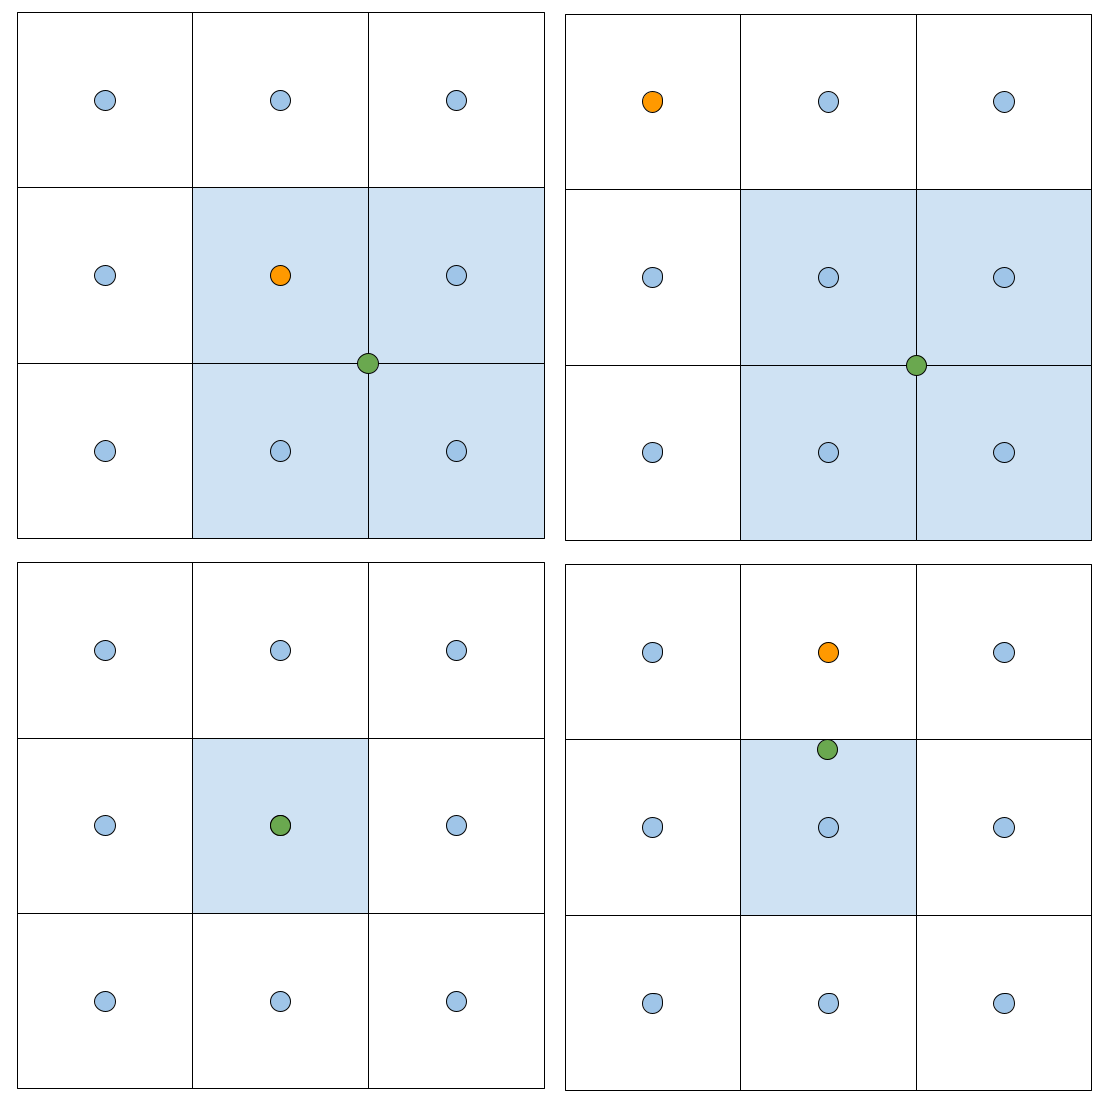
\includegraphics[width=0.5\linewidth]{../common/04_results/resources/detektion_min_und_max_fehler.png}
    \end{center}
    \caption{
        Extremsituationen zum Vergleich der Referenzposition und der wahren Position des Kugelmittelpunktes.
        Abgebildet ist ein Bildausschnitt mit 9 Pixeln. Die blauen Punkte sind die Pixelzentren, grün ist die wahre Position (subpixelgenau), orange ist die Referenzposition aus den Referenzdaten.
        Die Pixel rund um die wahre Position sind blau hinterlegt.
        Oben-Links: Der maximale Fehler ist eine halbe Pixeldiagonale, wenn die wahre Position zwischen vier Pixeln liegt und die Referenzposition einem der Pixel rund um die tatsächliche Position entspricht.
        Unten-Links: Der minimale Fehler ist $0$, wenn die wahre Position genau dem Pixelzentrum entspricht und dieses Pixel in den Referenzdaten ausgewählt wurde.
        Oben-Rechts: Der maximale Fehler ist 1.5 Pixeldiagonalen, wenn die wahre Position zwischen vier Pixeln liegt und die Referenzposition um ein Pixel daneben ist.
        Unten-Rechts: Der minimale Fehler ist eine halbe Pixelbreite/-höhe wenn die wahre Position innerhalb des zentralen Pixels liegt und die Referenzposition um ein Pixel falsch daneben ist.
    }
    \label{fig:detektion_resultate_min_max_fehler_referenzdaten}
\end{figure}

In Abschnitt \ref{kap:tracking} wurde beschrieben, dass in der Live-Detektion eine Stabilisierung der detektierten Positionen
über die Zeit durchgeführt wird.
In diesem Kapitel wurden nur Bilder für den Vergleich zwischen Detektion und Realität verwendet, wodurch es sich um Momentaufnahmen handelt.
Es kann sein, dass die Stabilisierung in gewissen Fällen die detektierten Positionen verbessert,
weil Positionsfehler in einzelnen Bilder geglättet werden.
